\section{Evaluation} \label{sec:evaluation}
The purpose of the evaluation is to establish knowledge concerning the possibility of creating a video game AI that matches the player's performance through the use of a genetic algorithm; as stated in the final problem statement.(See section XX)


\subsection{Method}
the method of testing and evaluating said results will be constructed in the following manner.

Test subjects will be asked to play several games/levels of the product prototype whereof each game represent a new improved generation of our genetic algorithm. The general purpose is to account for the effectiveness of our genetic algorithm and the used method of alternations between the various states of the finite state machine, to evaluate whether our genetic algorithm is actually matching player performance.

There are several aspects that must be accounted for:

\begin{itemize}
\item How is player performance considered matched?
\item does our implementation of alternation between the various states of a finite state machine match player performance?
\end{itemize}


\textbf{Player Performance specification}


In section \ref{ssec:player-performance}, assessment of player performance is considered, and the following allegation of defining player performance matched, is specified as such;

The player performance will be considered matched if the attained score(points) of each game/generation of one single test participant is either equal or lower than the previous attained score(points acquired).

\textbf{Pre test specification}


A pre test of the prototype will be conducted to ensure that the implemented parameters of the prototype is optimal for testing to successfully answer to the final problem statement.
Additionally the pre test will determine the number of simulations and generations that will be used throughout a single test of one single test participant.

\textbf{Main Test specification}

The test will consist of test participants playing levels of the prototype where each level is consisting of a new generation of the genetic algorithm.

The statistical test method and output data evaluation thereof will be conducted in accordance with the procedure listed by Field and Hole, 2003 \cite[pp. 265-277]{Field2003}, of how to design an experiment.

\begin{itemize}
\item Collected data: Scores

The data collected will consists of points(points collected throughout a single level played in the prototype) which can be categorized as interval data.
\item Independent variable(s)

One independent variable will be modified, and is the alternation between the various states of the finite state machine in the prototype, as specified in the final problem statement.(See section XX)
\item experimental design

The experiment is considered of type experimental, as we look for differences between conditions which is the alternations of the independent variable.
\item repeated measures

Each participant will participate in each condition of the experiment and provide scores to each, and the design is therefore considered a repeated measure design.
\item Parametric data

The data is considered parametric as the collected data is of type interval data. as described by Field and Hole, 2003 \cite[pp. 269]{Field2003}, the variation of scores in each condition of the test is somewhat comparable.

\end{itemize}


\subsection{Pre Test}

\subsubsection{Pre Test Purpose}
\subsubsection{Pre Test Method}
\subsubsection{Pre Test Procedure}
\subsubsection{Pre Test Results}
\subsubsection{Pre Test Result evaluation}

\subsection{Procedure}

\newpage
\subsection{Test Data and Results}
The following content is the combined data collected from the conducted test accompanied by a description of content.

\subsubsection{Main test data}
The acquired main test data consist of the following content(See figure \ref{fig:testdata} for data snippet).

The entire list of recorded data can be accessed in the digital appendix.

\begin{figure}[!htbp]
\centering
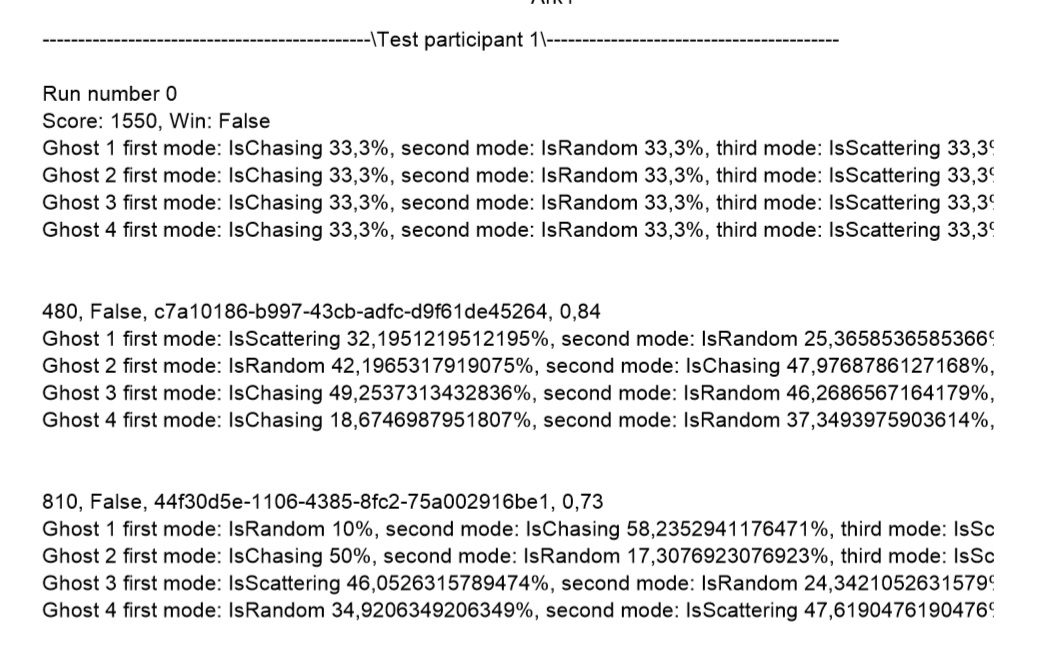
\includegraphics[scale=0.5]{testdata.jpg}
\caption{test data representation}
\label{fig:testdata}
\end{figure}


\newpage

The collected data consists of the following elements in descending order:

\begin{itemize}
\item  \textbf{Text participant}

Represent the participant number running from 1-21.
\item  \textbf{Run number}

Represent the current generation that the test participant is currently playing. Ranges from 0-9.
\item  \textbf{Score}

Represent the amount of points attained in the current generation/level.
\item  \textbf{Win}

Represent whether or not the test participant won the generation/level in a boolean statement. Win:True is the player won and Win:False is the player lost.
\item  \textbf{Ghost Mode}

Ghost 1-4 mode represent each of the four ghosts.


IsChasing, isRandom and isScattering represent the ghost Modes.(See section XX for mode description)

The percentages represent the length that each mode is active.

the order(sequence of modes) of each ghosts represent the order that the MonsterModes are switched between.(See section XX for documentation) Changing the order of the modes will change the time they are active during play or simulation in the prototype.
\end{itemize}

\newpage
Figure \ref{fig:testdata_simulation} depicts the data acquired of the simulations. After each level/generation played by a test participant there are 10 simulations.
The data recorded consists of the following elements for each simulation:

\begin{figure}[!htbp]
\centering
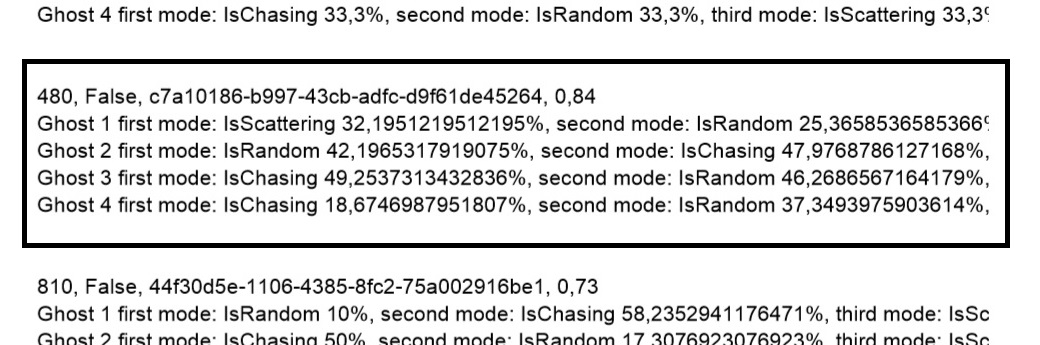
\includegraphics[scale=0.5]{testdata_simulation.jpg}
\caption{test data representation: Simulation}
\label{fig:testdata_simulation}
\end{figure}

\begin{itemize}
\item \textbf{first occurring number}

Represents the points collected during the entire simulation.

\item  \textbf{false/true}

Similar to the played level/generation, the boolean describes if the level is won or lost.

\item \textbf{<listCycles>}

The list represents the genes within each chromosome which are the solution to the given simulation.

\item \textbf{Fitness score}

The number ranging from 0-1 is the assigned fitness score to the current simulation. Depicted as 0.84 in the snippet(See figure \ref{fig:testdata_simulation})
\end{itemize}
\newpage
\subsubsection{Player level/generation points}
The following snippet(See figure \ref{fig:point_collection}) depicts the points collected by each one of the test participants from each generation/level.

The rows is the points collected from all test participants for each generation/level.

The columns are points collected by each test participant over the course of playing against the improved genetic algorithm over 10 generations. Ranging from generation 0 to generation 9(GEN 0 - GEN 9).
\begin{figure}[!htbp]
\centering
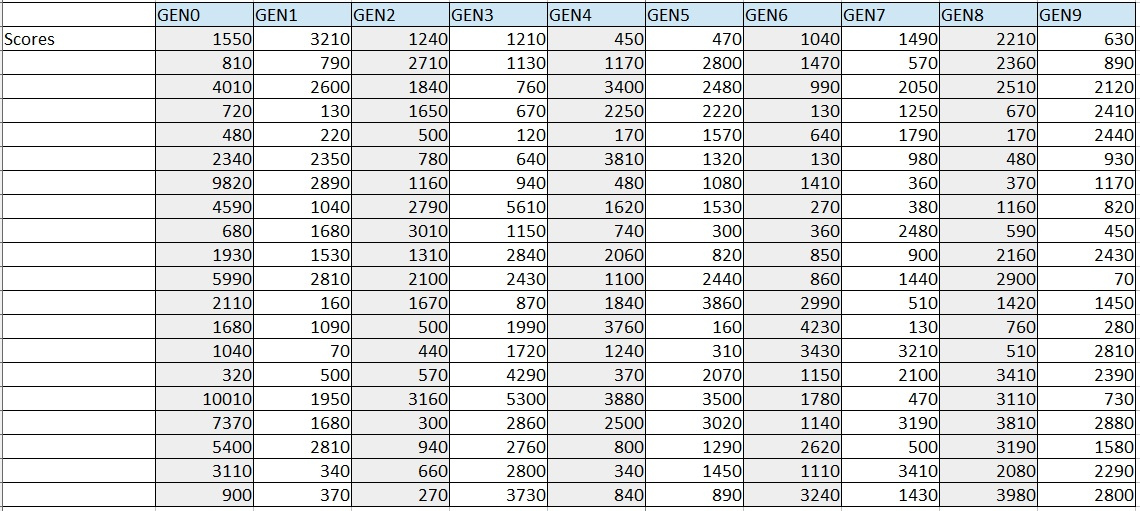
\includegraphics[scale=0.5]{player_points.jpg}
\caption{point collection}
\label{fig:point_collection}
\end{figure}

\subsubsection{Questionnaire data}



\subsection{Result evaluation}
\subsection{Evaluation discussion}